\documentclass[11pt,a4paper]{article}
\usepackage[margin=2.3cm]{geometry}
\usepackage[T1]{fontenc}
\usepackage{textcomp}
\input{glyphtounicode}
\pdfgentounicode=1
\usepackage{lmodern}
\usepackage{amsmath}
\usepackage{xcolor}
\usepackage{listings}
\usepackage{tcolorbox}
\tcbuselibrary{breakable}
\usepackage{booktabs}
\usepackage{array}
\usepackage{tikz}
\usetikzlibrary{decorations.pathreplacing}
\usepackage{float}
\usepackage{graphicx}
\graphicspath{{images/}}
\usepackage{hyperref}
\hypersetup{colorlinks=true, linkcolor=blue!50!black, citecolor=green!40!black}

\usepackage{accsupp}
% line numbers are drawn but excluded from copied text
\newcommand{\nocopy}[1]{\BeginAccSupp{method=escape,ActualText={}}#1\EndAccSupp{}}
\lstset{
  language=C, basicstyle=\ttfamily\small, keywordstyle={}, commentstyle={}, stringstyle={},
  numbers=left, numberstyle=\footnotesize\nocopy, numbersep=10pt, xleftmargin=2.4em,
  frame=none, columns=fullflexible, keepspaces=true, upquote=true, showstringspaces=false,
  breaklines=true, captionpos=b, aboveskip=1em, belowskip=0.8em
}
\lstdefinestyle{sh}{language=bash, numbers=none, xleftmargin=2.4em}
\renewcommand{\lstlistingname}{Listing}
% code names in the text: grey monospace
\let\origtexttt\texttt
\renewcommand{\texttt}[1]{\textcolor{black!60}{\origtexttt{#1}}}

\newtcolorbox{keyidea}{colback=blue!4, colframe=blue!45!black, title=Key ideas, fonttitle=\bfseries\small}
\newtcolorbox{experiment}{breakable, colback=orange!5, colframe=orange!70!black, title=Experiment, fonttitle=\bfseries\small}
\title{\textbf{OpenMP GPU Teams and Threads: \texttt{num\_teams} and \texttt{thread\_limit}}\\[4pt]\large Lesson 32: how much parallelism a GPU needs}
\author{Gustavo Lozano}
\date{November 2026}

\begin{document}
\maketitle

\noindent\textit{\small Source: Deakin \& Mattson~\cite{dm}, Ch.~5 (Using a GPU Effectively) and
Ch.~6 (Managing a GPU's Hierarchical Parallelism). Prerequisite: \texttt{00-openmp\_target\_data.pdf}
(Lesson 31).}

\section{The idea}
The GTX 1050 has 5 \emph{streaming multiprocessors} (SMs) with 128 cores each
(Figure~\ref{fig:sm}).
\begin{itemize}
  \item A \textbf{team} runs on one SM and never spans two; one SM can hold several teams.
  \item The threads of a team run in groups of 32, called \textbf{warps}, that execute the same
        instruction together.
  \item A read from GPU memory takes hundreds of cycles. While one warp waits, the SM runs
        another. So an SM is only busy if it holds many warps: up to 2048 threads per SM,
        $5\times2048 = 10\,240$ for the whole GPU.
\end{itemize}
Too few teams leave SMs idle; too few threads leave each SM waiting for memory.

\begin{figure}[H]
\centering
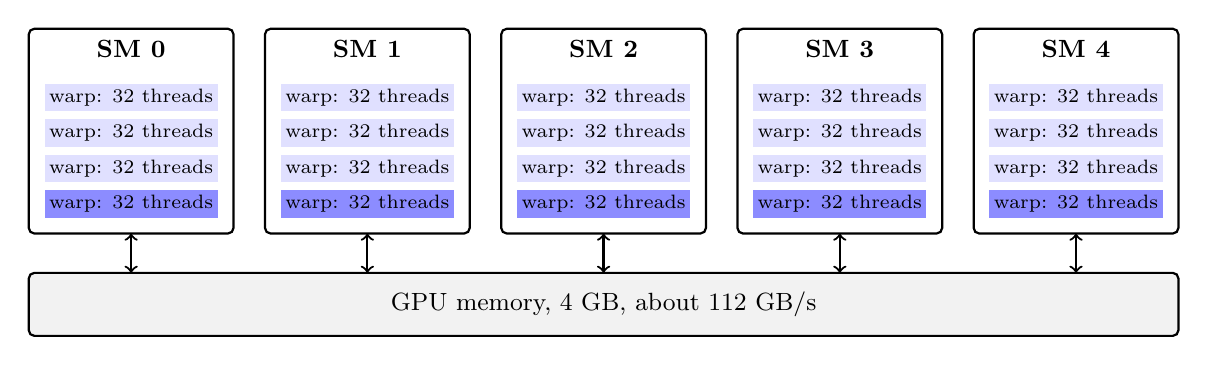
\begin{tikzpicture}[font=\small]
  \foreach \s in {0,...,4} {
    \begin{scope}[xshift=\s*3cm]
      \draw[thick, rounded corners=2pt] (0,0) rectangle (2.6,2.6);
      \node[font=\small\bfseries] at (1.3,2.35) {SM \s};
      \foreach \w in {0,...,3} {
        \pgfmathsetmacro{\c}{\w==0 ? 45 : 12}
        \fill[blue!\c] (0.2,0.2+0.45*\w) rectangle (2.4,0.55+0.45*\w);
        \node[font=\scriptsize] at (1.3,0.375+0.45*\w) {warp: 32 threads};
      }
    \end{scope}
  }
  \draw[thick, fill=black!5, rounded corners=2pt] (0,-1.3) rectangle (14.6,-0.5);
  \node at (7.3,-0.9) {GPU memory, 4 GB, about 112 GB/s};
  \foreach \s in {0,...,4} \draw[<->, thick] (1.3+3*\s,-0.5) -- (1.3+3*\s,0);
\end{tikzpicture}
\caption{The GTX 1050: 5 SMs. Each SM switches between its warps (dark: the warp running now;
light: warps waiting for memory). Teams are placed on the SMs; a team's threads form warps.}
\label{fig:sm}
\end{figure}

\section{The clauses}
\begin{lstlisting}[numbers=none]
#pragma omp target teams distribute parallel for \
        num_teams(T) thread_limit(N)
\end{lstlisting}
\begin{itemize}
  \item \texttt{num\_teams(T)}: use at most $T$ teams;
  \item \texttt{thread\_limit(N)}: use at most $N$ threads per team (a multiple of 32 fills
        whole warps).
\end{itemize}
Both are upper bounds; without them the compiler and runtime choose, usually well. Inside the
loop, \texttt{omp\_get\_num\_teams()} and \texttt{omp\_get\_num\_threads()} report what a launch
really used.

\section{The code}
The kernel $y = 2x$ on $2^{25}$ doubles is launched with different numbers of teams and threads
(\texttt{scale}, lines 23--48). \texttt{x} and \texttt{y} stay on the GPU (Lesson 31), so only
the kernel is timed; each line is the best of 10 launches. Bandwidth counts 16 bytes per
element: read $x$, write $y$.
\begin{itemize}
  \item Part A (line 81): 256 threads per team, from 1 to 2560 teams.
  \item Part B (line 86): 5 teams, one per SM, from 32 to 1024 threads each.
\end{itemize}

\begin{lstlisting}[caption={\textbf{\origtexttt{target\_teams.c}} -- the same kernel launched with different numbers of teams and threads.}, label={lst:teams}]
/*
 * target_teams.c -- OpenMP Lesson 32: how many teams and threads on the GPU,
 * with num_teams and thread_limit.
 * Source: Deakin & Mattson (2023), Ch. 5 (Using a GPU Effectively) and
 *         Ch. 6 (Managing a GPU's Hierarchical Parallelism).
 *
 * The same kernel y = 2 x runs with different numbers of teams and threads
 * per team.  x and y stay on the GPU; each launch is timed (best of NREP).
 *
 * Compile:  clang -O2 -fopenmp --offload-arch=sm_61 \
 *                 -o target_teams target_teams.c
 * Run:      OMP_TARGET_OFFLOAD=MANDATORY ./target_teams [log2 n]
 */

#include <stdio.h>
#include <stdlib.h>
#include <omp.h>

#define NREP 10

/* y = 2 x with nteams teams of at most nthreads threads; 0 = let the
   runtime choose.  info[] returns what was actually used.              */
static void scale(const double *x, double *y, long n,
                  int nteams, int nthreads, int *info)
{
    if (nteams > 0) {
        #pragma omp target teams distribute parallel for \
                num_teams(nteams) thread_limit(nthreads) \
                map(present, alloc: x[0:n], y[0:n]) map(from: info[0:2])
        for (long i = 0; i < n; i++) {
            y[i] = 2.0 * x[i];
            if (i == 0) {                      /* what the launch really used */
                info[0] = omp_get_num_teams();
                info[1] = omp_get_num_threads();
            }
        }
    } else {
        #pragma omp target teams distribute parallel for \
                map(present, alloc: x[0:n], y[0:n]) map(from: info[0:2])
        for (long i = 0; i < n; i++) {
            y[i] = 2.0 * x[i];
            if (i == 0) {                      /* what the launch really used */
                info[0] = omp_get_num_teams();
                info[1] = omp_get_num_threads();
            }
        }
    }
}

/* best time of NREP launches; prints teams, threads and bandwidth */
static void measure(const double *x, double *y, long n, int nteams, int nthreads)
{
    int info[2] = {0, 0};
    double best = 1e30;
    for (int r = 0; r < NREP; r++) {
        double t = omp_get_wtime();
        scale(x, y, n, nteams, nthreads, info);
        t = omp_get_wtime() - t;
        if (t < best) best = t;
    }
    printf("%7d %8d %10ld %9.2f %8.1f\n", info[0], info[1],
           (long)info[0] * info[1], 1e3 * best, 16.0 * n / best / 1e9);
}

int main(int argc, char **argv)
{
    long n = 1L << (argc > 1 ? atoi(argv[1]) : 25);   /* 2^25 doubles = 256 MiB */
    double *x = malloc(n * sizeof(double));
    double *y = malloc(n * sizeof(double));
    for (long i = 0; i < n; i++) x[i] = 1.0;

    #pragma omp target enter data map(to: x[0:n]) map(alloc: y[0:n])

    printf("n = %ld doubles; 16 bytes per element (read x, write y)\n", n);
    printf("  teams  threads      total        ms     GB/s\n");

    printf("runtime default:\n");
    measure(x, y, n, 0, 0);

    printf("A. 256 threads per team, more and more teams:\n");
    int teams[] = {1, 2, 5, 10, 20, 40, 80, 160, 640, 2560};
    for (int k = 0; k < 10; k++)
        measure(x, y, n, teams[k], 256);

    printf("B. 5 teams (one per multiprocessor), more and more threads:\n");
    int threads[] = {32, 64, 128, 256, 512, 1024};
    for (int k = 0; k < 6; k++)
        measure(x, y, n, 5, threads[k]);

    #pragma omp target exit data map(from: y[0:n]) map(delete: x[0:n])
    long bad = 0;
    for (long i = 0; i < n; i++) bad += (y[i] != 2.0);
    printf("correct: %s\n", bad ? "NO" : "yes");
    free(x); free(y);
    return 0;
}
\end{lstlisting}

\begin{lstlisting}[style=sh]
clang -O2 -fopenmp --offload-arch=sm_61 -o target_teams target_teams.c
OMP_TARGET_OFFLOAD=MANDATORY ./target_teams
\end{lstlisting}

\begin{keyidea}
\begin{itemize}
  \item A team runs on one SM; its threads run in warps of 32.
  \item The GPU hides memory latency by switching warps, so it needs thousands of threads in
        flight: here about $10^4$.
  \item \texttt{num\_teams} and \texttt{thread\_limit} are upper bounds; check what was used
        with \texttt{omp\_get\_num\_teams()} and \texttt{omp\_get\_num\_threads()}.
  \item The default is usually good; change it only after measuring.
\end{itemize}
\end{keyidea}

\section{The experiment}
\begin{experiment}
\textbf{Question:} how many threads does the GPU need to reach its memory bandwidth?

Run the program:
\begin{lstlisting}[style=sh]
OMP_TARGET_OFFLOAD=MANDATORY ./target_teams
\end{lstlisting}

\textbf{What to observe and answer.}
\begin{enumerate}
  \item How many teams and threads does the runtime choose by default, and what bandwidth does
        it reach?
  \item In part A, why is one team so slow? From how many teams (total threads) does the
        bandwidth stop growing?
  \item In part B every SM is in use. Why does the bandwidth still grow with the threads per team?
\end{enumerate}
\end{experiment}

\paragraph{Answers (read after trying).}

\noindent(1)~The runtime sizes the launch from the loop length: many teams of 128 to 256
threads, so it should reach close to the best bandwidth of part A.

\noindent(2)~One team runs on one SM: 4 of the 5 SMs are idle, and the one in use has only 8
warps to hide the memory latency. The bandwidth grows with the number of teams until about
$10^4$ threads are in flight (about 40 teams of 256) and then stays flat near the memory
bandwidth; more teams only wait their turn.

\noindent(3)~With 32 threads per team each SM has a single warp: whenever it waits for memory,
the SM has nothing else to run. More warps per SM overlap more memory requests, so the
bandwidth grows until the latency is hidden.

\paragraph{Next lesson.} Lesson 33: the order of memory accesses on the GPU (coalescing).

\begin{thebibliography}{9}
\bibitem{dm} T.~Deakin and T.~G.~Mattson. \emph{Programming Your GPU with OpenMP: Performance
  Portability for GPUs}. MIT Press, Cambridge, MA, 2023.
\end{thebibliography}
\end{document}
